\documentclass[border=3pt]{standalone}
\usepackage[T1]{fontenc}
\AtBeginDocument{\hyphenpenalty=10000 \exhyphenpenalty=10000 \pretolerance=-1 \tolerance=9999}
\usepackage{helvet}
\renewcommand{\familydefault}{\sfdefault}
\usepackage{amsmath,amssymb}
\usepackage[eulergreek]{sansmath}
\sansmath
\usepackage{tikz}
\usetikzlibrary{positioning,arrows.meta,calc,shapes.geometric,shapes.symbols,shapes.misc,backgrounds,patterns,decorations.pathreplacing,shadows.blur}
% ---------------- palette (distinct from the earlier manuscript)
\definecolor{ink}{HTML}{1D2B3A}
\definecolor{mute}{HTML}{6B7280}
\definecolor{line}{HTML}{CBD2D9}
\definecolor{sand}{HTML}{F7F3EC}
\definecolor{cor}{HTML}{E76F51}   % Stage 1 (endoscopy)
\definecolor{corl}{HTML}{FCE9E3}
\definecolor{sea}{HTML}{2A9D8F}   % Stage 2 (CT, PET, genomics)
\definecolor{seal}{HTML}{E0F2EF}
\definecolor{gold}{HTML}{D9A42B}  % data-integrity audits
\definecolor{goldl}{HTML}{FBF1D9}
\definecolor{nav}{HTML}{264653}   % reliability layer
\definecolor{navl}{HTML}{E3EAEE}
\definecolor{plum}{HTML}{8E5572}  % outputs to clinician
\definecolor{pluml}{HTML}{F3E8EE}
\tikzset{
  >={Stealth[length=2.4mm,width=1.8mm]},
  flow/.style={->, line width=0.9pt, draw=ink!70},
  thin/.style={->, line width=0.6pt, draw=mute},
  card/.style={draw=#1, line width=0.7pt, fill=white, rounded corners=3pt, blur shadow={shadow blur steps=5, shadow xshift=0.4mm, shadow yshift=-0.4mm, shadow opacity=18}},
  tag/.style={fill=#1, text=white, font=\tiny\bfseries, rounded corners=1.6pt, inner sep=1.6pt},
  hdr/.style={font=\scriptsize\bfseries, text=#1},
  sm/.style={font=\tiny, text=ink, align=center},
  smm/.style={font=\tiny, text=mute, align=center},
  num/.style={circle, fill=#1, text=white, font=\tiny\bfseries, inner sep=0.9pt, minimum size=4mm},
}

\graphicspath{{../assets/}}
\begin{document}
\begin{tikzpicture}[x=1mm,y=1mm]
% ============ background
\fill[sand, rounded corners=4pt] (-2,-9) rectangle (182,107);
% ============ clinical pathway (chevrons)
\node[font=\scriptsize\bfseries, text=ink, anchor=west] at (0,103) {Clinical pathway};
\foreach \i/\t/\c/\sh in {0/Upper GI endoscopy/mute/45, 1/Barrett's esophagus?/cor/100, 2/Surveillance entry/cor/70, 3/Carcinoma diagnosed/mute/45, 4/Histological subtype/sea/100, 5/Treatment planning/mute/45} {
  \node[signal, signal to=east, signal from=west, signal pointer angle=120, fill=\c!\sh, text=white, font=\tiny\bfseries,
        minimum width=29mm, minimum height=6.2mm, inner sep=1pt, anchor=west] at ({\i*30},96) {\t};
}
% ============ column headers
\foreach \x/\n/\t/\c in {16/1/Data audit/gold, 58/2/Representation and model/ink, 100/3/Reliability layer/nav, 142/4/Outcome and evidence/plum} {
  \node[num=\c] at (\x+3,86) {\n};
  \node[font=\scriptsize\bfseries, text=\c!85!black, anchor=west] at (\x+6.5,86) {\t};
  \draw[\c, line width=1.2pt] (\x,83) -- (\x+38,83);
}
% ============ row tabs
\foreach \y/\c/\t/\s in {48/cor/Stage 1/white light endoscopy, 7/sea/Stage 2/{CT, PET, genomics}} {
  \fill[\c, rounded corners=3pt] (0,\y) rectangle (12,\y+33);
  \node[rotate=90, text=white, font=\scriptsize\bfseries] at (4.6,\y+16.5) {\t};
  \node[rotate=90, text=white, font=\tiny] at (8.8,\y+16.5) {\s};
}
% ============ cards
\foreach \x/\c in {16/gold, 58/ink, 100/nav, 142/plum} {
  \foreach \y in {48, 7} { \node[card=\c!70, minimum width=38mm, minimum height=33mm, anchor=south west] at (\x,\y) {}; }
}
% arrows between columns
\foreach \y in {64.5, 23.5} { \foreach \x in {54.6, 96.6, 138.6} { \draw[flow] (\x,\y) -- (\x+3,\y); } }

% ---------------- Stage 1 glyphs and text
% (1) duplicate audit: original + copy linked
\begin{scope}[shift={(35,70)}]
  \node[inner sep=0pt] at (-7.5,0) {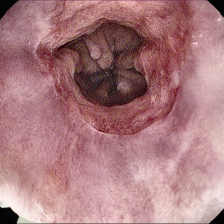
\includegraphics[width=11mm]{s1_dup_orig.png}};
  \node[inner sep=0pt] at (7.5,0) {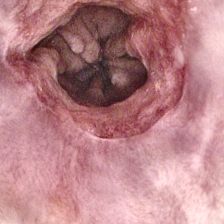
\includegraphics[width=11mm]{s1_dup_aug.png}};
  \draw[gold, line width=1.1pt] (-1.6,0.9) -- (1.6,0.9) (-1.6,-0.9) -- (1.6,-0.9);
  \node[tag=gold] at (0,8.2) {cos = 1.00};
  \node[smm] at (-7.5,-7.2) {original}; \node[smm] at (7.5,-7.2) {augmented copy};
\end{scope}
\node[sm, text width=36mm] at (35,56.5) {\textbf{Duplicate audit}\\every image linked to its augmented copy (1,017 pairs);\\splits grouped by source image};
% (2) multiscale + encoder
\begin{scope}[shift={(77,70)}]
  \node[inner sep=0pt] at (-13.6,0.5) {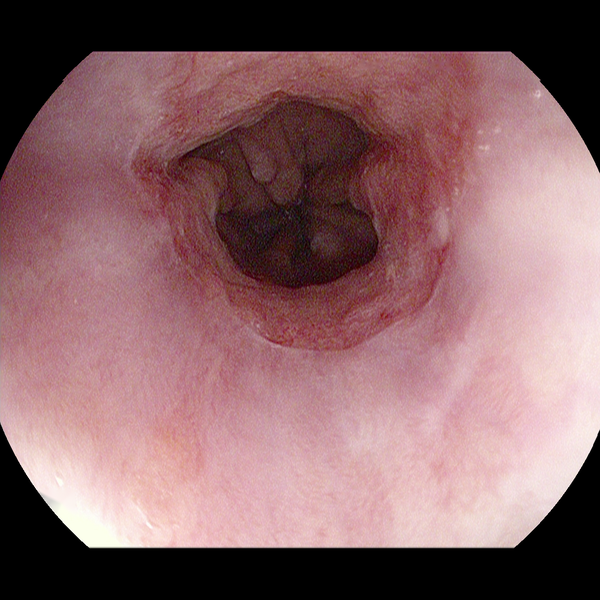
\includegraphics[width=8mm]{s1_raw.png}};
  \draw[mute, line width=0.5pt, -{Stealth[length=0.9mm,width=0.9mm]}] (-9.4,0.5) -- (-7.7,0.5);
  \node[inner sep=0pt] at (-4.9,0.5) {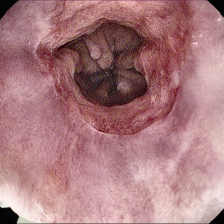
\includegraphics[width=5.2mm]{s1_v00.png}};
  \node[inner sep=0pt] at (0.6,0.5) {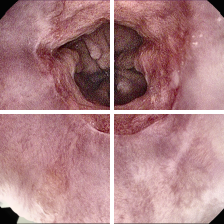
\includegraphics[width=5.2mm]{s1_quadmosaic.png}};
  \node[inner sep=0pt] at (6.1,0.5) {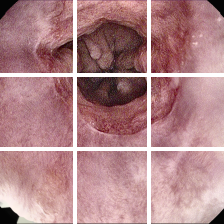
\includegraphics[width=5.2mm]{s1_tilemosaic.png}};
  \node[smm] at (0.6,5.6) {14 multiscale views};
  \node[font=\fontsize{4}{4.5}\selectfont, text=mute] at (-4.9,-3.2) {1}; \node[font=\fontsize{4}{4.5}\selectfont, text=mute] at (0.6,-3.2) {4}; \node[font=\fontsize{4}{4.5}\selectfont, text=mute] at (6.1,-3.2) {9};
  \node[trapezium, trapezium angle=70, shape border rotate=270, fill=ink!85, minimum width=8mm, minimum height=6.4mm, inner sep=0.5pt] at (14.6,0.5) {};
  \node[text=white, font=\fontsize{4}{4.5}\selectfont\bfseries] at (14.6,0.5) {DINOv2};
  \draw[mute, line width=0.5pt, -{Stealth[length=0.9mm,width=0.9mm]}] (8.9,0.5) -- (10.7,0.5);
\end{scope}
\node[sm, text width=36mm] at (77,56.5) {\textbf{Frozen foundation features}\\14 multiscale views, DINOv2 ViT-B/14;\\mean pooling, ensemble of 25 members};
% (3) reliability gauge + set
\begin{scope}[shift={(119,70)}]
  \foreach \a/\c in {180/sea, 150/sea!60, 120/gold, 90/gold!80, 60/cor!70, 30/cor} { \fill[\c] (-6,0) -- ++(\a:6) arc (\a:\a-30:6) -- cycle; }
  \fill[white] (-6,0) circle (3.2);
  \draw[ink, line width=1pt] (-6,0) -- ++(128:5.4); \fill[ink] (-6,0) circle (0.7);
  \node[smm] at (-6,-2.4) {uncertainty};
  \node[draw=nav, line width=0.7pt, rounded corners=2pt, font=\tiny\bfseries, text=nav, inner sep=1.6pt] at (7,2.2) {\{BE\}};
  \node[draw=nav, line width=0.7pt, dashed, rounded corners=2pt, font=\tiny\bfseries, text=nav, inner sep=1.6pt] at (7,-2.6) {\{BE, N\}};
  \node[smm] at (7,-6.2) {conformal sets};
\end{scope}
\node[sm, text width=36mm] at (119,56.5) {\textbf{Calibrated output with deferral}\\Platt calibration, epistemic deferral,\\class conditional conformal sets,\\shift monitor};
% (4) evidence: ROC glyph
\begin{scope}[shift={(152,63)}]
  \draw[line, line width=0.4pt] (0,0) rectangle (13,13); \draw[mute, dashed, line width=0.3pt] (0,0)--(13,13);
  \draw[cor, line width=1pt] (0,0) .. controls (0.6,8.5) and (3,11.6) .. (13,13);
  \draw[cor!55, line width=1pt] (0,0) .. controls (1.4,7) and (4.2,10.4) .. (13,13);
\end{scope}
\node[font=\tiny, text=ink, anchor=west, align=left] at (166.5,72.5) {\textbf{0.914}\\[-1pt]internal};
\node[font=\tiny, text=ink, anchor=west, align=left] at (166.5,65.5) {\textbf{0.872}\\[-1pt]external};
\node[sm, text width=36mm] at (161,56.5) {\textbf{Evaluation free of leakage}\\grouped internal test (204 images);\\GastroVision, all settings frozen};

% ---------------- Stage 2 glyphs and text
% (1) missingness audit matrix
\begin{scope}[shift={(28,24)}]
  \foreach \r/\lab/\cnt in {2/G/18, 1/CT/4, 0/PET/1} {
    \node[smm, anchor=east] at (-0.6,\r*3.2+1.2) {\lab};
    \foreach \k in {0,...,19} { \pgfmathsetmacro{\f}{(\k<\cnt) ? 1 : 0}
      \ifdim\f pt>0.5pt \fill[sea] (\k*0.75,\r*3.2) rectangle ++(0.6,2.4); \else \draw[line, line width=0.3pt] (\k*0.75,\r*3.2) rectangle ++(0.6,2.4); \fi }
  }
  \node[tag=gold] at (20.8,8.3) {gate};
\end{scope}
\node[sm, text width=36mm] at (35,15.5) {\textbf{Missingness audit}\\does availability alone predict the label?\\subtype passes; staging excluded};
% (2) tokens + attention
\begin{scope}[shift={(77,29.5)}]
  \node[inner sep=0pt] at (-12,1) {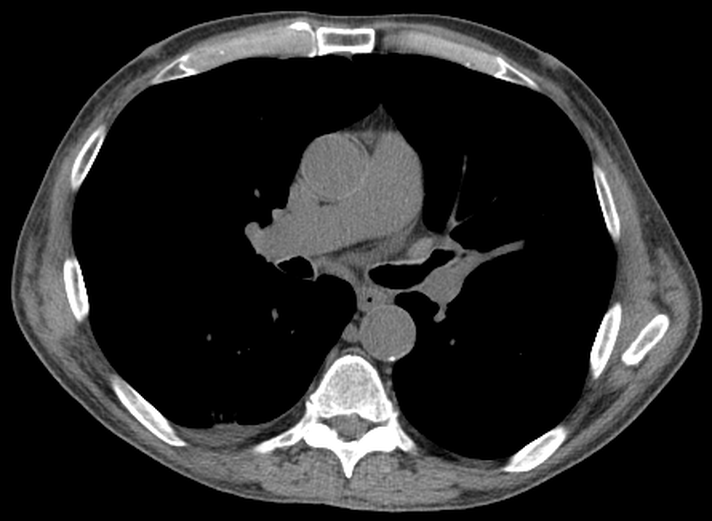
\includegraphics[width=10.4mm]{s2_ct.png}};
  \node[inner sep=0pt] at (-0.6,1) {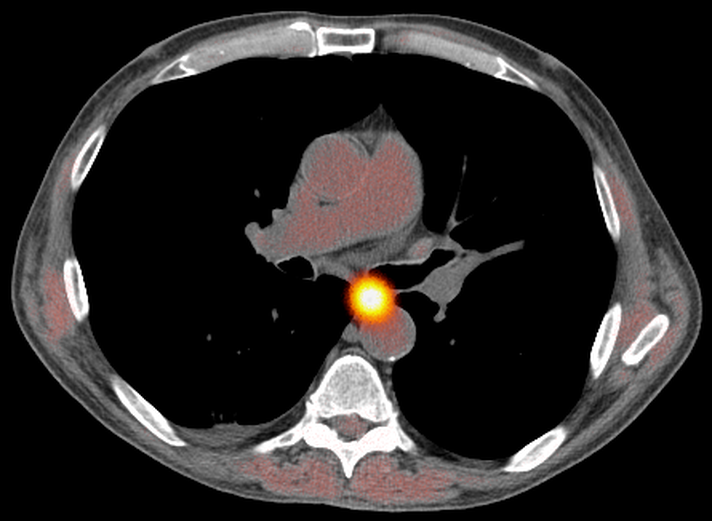
\includegraphics[width=10.4mm]{s2_pet.png}};
  \node[inner sep=0pt] at (10.8,1) {
\includegraphics[width=10.4mm]{s2_geno.png}};
  \node[smm] at (-12,-4.6) {CT (34)}; \node[smm] at (-0.6,-4.6) {PET (5)}; \node[smm] at (10.8,-4.6) {genomics (180)};
  \node[smm] at (-0.6,6.9) {three modalities, any subset};
\end{scope}
\node[sm, text width=36mm] at (77,15.5) {\textbf{Fusion with missing modalities}\\CT, PET and genomic tokens;\\key padding mask, any subset scored};
% (3) ablation bars
\begin{scope}[shift={(110,22)}]
  \fill[sea] (-2,0) rectangle (1.5,10.2); \fill[sea!45] (5,0) rectangle (8.5,10.1);
  \draw[mute, line width=0.4pt] (-3,0) -- (10,0);
  \node[smm] at (-0.25,-2) {fusion}; \node[smm] at (6.75,-2) {genomics};
  \node[smm] at (3.25,12.4) {$p$ = 0.742};
  \fill[nav] (15,9) circle (1.1); \fill[nav!55] (19,9) circle (1.1); \fill[nav!25] (23,9) circle (1.1);
  \node[smm] at (19,5.6) {modality dropout};
\end{scope}
\node[sm, text width=36mm] at (119,15.5) {\textbf{Controlled comparison}\\ablation with genomics only, DeLong test,\\modality dropout during training};
% (4) nested CV ring
\begin{scope}[shift={(155,26)}]
  \foreach \k/\sh in {0/100,1/30,2/30,3/30,4/30} { \fill[sea!\sh] (0,0) -- ({90-\k*72}:6.2) arc ({90-\k*72}:{90-(\k+1)*72+4}:6.2) -- cycle; }
  \fill[white] (0,0) circle (3.4);
  \node[font=\tiny\bfseries, text=ink] at (0,0) {3$\times$5};
\end{scope}
\node[font=\tiny, text=ink, anchor=west, align=left] at (164,28.5) {\textbf{0.870}\\[-1pt]subtype};
\node[font=\tiny, text=ink, anchor=west, align=left] at (164,21.5) {\textbf{199}\\[-1pt]patients};
\node[sm, text width=36mm] at (161,15.5) {\textbf{Nested cross validation}\\every patient scored by models\\that never saw that patient};

% ============ decision banner
\fill[plum!12, rounded corners=3pt] (16,-7.5) rectangle (180,2.6);
\node[font=\scriptsize\bfseries, text=plum!85!black, anchor=west] at (18,-2.4) {Decision support};
\node[font=\tiny, text=ink, anchor=west] at (44,-2.4) {\textbf{accept} a single confident label \quad$\boldsymbol{\cdot}$\quad \textbf{defer} to the clinician when the conformal set is ambiguous, uncertainty is high or the input lies outside the training scope};
\end{tikzpicture}
\end{document}
